% !TEX root = ../main.tex

\section*{1}

Let denote LB and UB as a lower bound and upper bound of
of maximum number that an arbitrary line can intersect with a
triangulation $T$ of $n$. We claim that :

\begin{align*}
    \mathrm{LB} &= \text{No. Triangles in T} + 1\\
    \mathrm{UB} &= \text{No. Triangles in T} + 1
\end{align*}
\begin{figure}[h]
    \begin{center}
        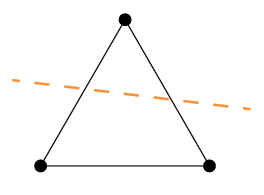
\includegraphics[width=0.5\textwidth]{smallest-triangulation}
        \caption{Smallest Triangulation}
        \label{fig:smallest-triangulation}
    \end{center}
\end{figure}

To prove LB, it is obvious to see from Figure \ref{fig:smallest-triangulation}
,the the smallest triangulation having 1 triangle, that the maximum number of intersection is $2$.
For UB, we have observed that for 1 triangle the number of intersetion is $2$.
which is the number of triangle plus 1. Let assume that for $k$ triangles
the max number of intersection is $k+1$. Next, if we add one more triangle,
one of its edges will be shared with the one of the old triangles, thus
it can generate only 1 more intersection. Thus, the number of max intersection
is $k+2$. Therefore, we can conclude that for a triangulation $T$ the $UB$ of
intersection between an arbitrary and $T$ equals to the number of triangles
in $T$ plus $1$ as we claim.

In naive approach of finding average intersection, traversing $n^2$ pairs and checking with all edges $O(n)$
takes $O(n^3)$ running time. To improve the efficiency, the data structure proven in Exercise Week 4 Question 3,
is used. Such that we can query the number of intersection between an arbitrary line and
edges in $O(\log{n})$ expected time.

Thus, we can find the average number of intersected edges with all lines through
a pair of input points.
